% Options for packages loaded elsewhere
\PassOptionsToPackage{unicode}{hyperref}
\PassOptionsToPackage{hyphens}{url}
%
\documentclass[
]{article}
\usepackage{amsmath,amssymb}
\usepackage{lmodern}
\usepackage{ifxetex,ifluatex}
\ifnum 0\ifxetex 1\fi\ifluatex 1\fi=0 % if pdftex
  \usepackage[T1]{fontenc}
  \usepackage[utf8]{inputenc}
  \usepackage{textcomp} % provide euro and other symbols
\else % if luatex or xetex
  \usepackage{unicode-math}
  \defaultfontfeatures{Scale=MatchLowercase}
  \defaultfontfeatures[\rmfamily]{Ligatures=TeX,Scale=1}
\fi
% Use upquote if available, for straight quotes in verbatim environments
\IfFileExists{upquote.sty}{\usepackage{upquote}}{}
\IfFileExists{microtype.sty}{% use microtype if available
  \usepackage[]{microtype}
  \UseMicrotypeSet[protrusion]{basicmath} % disable protrusion for tt fonts
}{}
\makeatletter
\@ifundefined{KOMAClassName}{% if non-KOMA class
  \IfFileExists{parskip.sty}{%
    \usepackage{parskip}
  }{% else
    \setlength{\parindent}{0pt}
    \setlength{\parskip}{6pt plus 2pt minus 1pt}}
}{% if KOMA class
  \KOMAoptions{parskip=half}}
\makeatother
\usepackage{xcolor}
\IfFileExists{xurl.sty}{\usepackage{xurl}}{} % add URL line breaks if available
\IfFileExists{bookmark.sty}{\usepackage{bookmark}}{\usepackage{hyperref}}
\hypersetup{
  pdftitle={Neural Networks and their Applications},
  pdfauthor={Keane Flynn},
  hidelinks,
  pdfcreator={LaTeX via pandoc}}
\urlstyle{same} % disable monospaced font for URLs
\usepackage[margin=1in]{geometry}
\usepackage{color}
\usepackage{fancyvrb}
\newcommand{\VerbBar}{|}
\newcommand{\VERB}{\Verb[commandchars=\\\{\}]}
\DefineVerbatimEnvironment{Highlighting}{Verbatim}{commandchars=\\\{\}}
% Add ',fontsize=\small' for more characters per line
\usepackage{framed}
\definecolor{shadecolor}{RGB}{248,248,248}
\newenvironment{Shaded}{\begin{snugshade}}{\end{snugshade}}
\newcommand{\AlertTok}[1]{\textcolor[rgb]{0.94,0.16,0.16}{#1}}
\newcommand{\AnnotationTok}[1]{\textcolor[rgb]{0.56,0.35,0.01}{\textbf{\textit{#1}}}}
\newcommand{\AttributeTok}[1]{\textcolor[rgb]{0.77,0.63,0.00}{#1}}
\newcommand{\BaseNTok}[1]{\textcolor[rgb]{0.00,0.00,0.81}{#1}}
\newcommand{\BuiltInTok}[1]{#1}
\newcommand{\CharTok}[1]{\textcolor[rgb]{0.31,0.60,0.02}{#1}}
\newcommand{\CommentTok}[1]{\textcolor[rgb]{0.56,0.35,0.01}{\textit{#1}}}
\newcommand{\CommentVarTok}[1]{\textcolor[rgb]{0.56,0.35,0.01}{\textbf{\textit{#1}}}}
\newcommand{\ConstantTok}[1]{\textcolor[rgb]{0.00,0.00,0.00}{#1}}
\newcommand{\ControlFlowTok}[1]{\textcolor[rgb]{0.13,0.29,0.53}{\textbf{#1}}}
\newcommand{\DataTypeTok}[1]{\textcolor[rgb]{0.13,0.29,0.53}{#1}}
\newcommand{\DecValTok}[1]{\textcolor[rgb]{0.00,0.00,0.81}{#1}}
\newcommand{\DocumentationTok}[1]{\textcolor[rgb]{0.56,0.35,0.01}{\textbf{\textit{#1}}}}
\newcommand{\ErrorTok}[1]{\textcolor[rgb]{0.64,0.00,0.00}{\textbf{#1}}}
\newcommand{\ExtensionTok}[1]{#1}
\newcommand{\FloatTok}[1]{\textcolor[rgb]{0.00,0.00,0.81}{#1}}
\newcommand{\FunctionTok}[1]{\textcolor[rgb]{0.00,0.00,0.00}{#1}}
\newcommand{\ImportTok}[1]{#1}
\newcommand{\InformationTok}[1]{\textcolor[rgb]{0.56,0.35,0.01}{\textbf{\textit{#1}}}}
\newcommand{\KeywordTok}[1]{\textcolor[rgb]{0.13,0.29,0.53}{\textbf{#1}}}
\newcommand{\NormalTok}[1]{#1}
\newcommand{\OperatorTok}[1]{\textcolor[rgb]{0.81,0.36,0.00}{\textbf{#1}}}
\newcommand{\OtherTok}[1]{\textcolor[rgb]{0.56,0.35,0.01}{#1}}
\newcommand{\PreprocessorTok}[1]{\textcolor[rgb]{0.56,0.35,0.01}{\textit{#1}}}
\newcommand{\RegionMarkerTok}[1]{#1}
\newcommand{\SpecialCharTok}[1]{\textcolor[rgb]{0.00,0.00,0.00}{#1}}
\newcommand{\SpecialStringTok}[1]{\textcolor[rgb]{0.31,0.60,0.02}{#1}}
\newcommand{\StringTok}[1]{\textcolor[rgb]{0.31,0.60,0.02}{#1}}
\newcommand{\VariableTok}[1]{\textcolor[rgb]{0.00,0.00,0.00}{#1}}
\newcommand{\VerbatimStringTok}[1]{\textcolor[rgb]{0.31,0.60,0.02}{#1}}
\newcommand{\WarningTok}[1]{\textcolor[rgb]{0.56,0.35,0.01}{\textbf{\textit{#1}}}}
\usepackage{graphicx}
\makeatletter
\def\maxwidth{\ifdim\Gin@nat@width>\linewidth\linewidth\else\Gin@nat@width\fi}
\def\maxheight{\ifdim\Gin@nat@height>\textheight\textheight\else\Gin@nat@height\fi}
\makeatother
% Scale images if necessary, so that they will not overflow the page
% margins by default, and it is still possible to overwrite the defaults
% using explicit options in \includegraphics[width, height, ...]{}
\setkeys{Gin}{width=\maxwidth,height=\maxheight,keepaspectratio}
% Set default figure placement to htbp
\makeatletter
\def\fps@figure{htbp}
\makeatother
\setlength{\emergencystretch}{3em} % prevent overfull lines
\providecommand{\tightlist}{%
  \setlength{\itemsep}{0pt}\setlength{\parskip}{0pt}}
\setcounter{secnumdepth}{-\maxdimen} % remove section numbering
\ifluatex
  \usepackage{selnolig}  % disable illegal ligatures
\fi

\title{Neural Networks and their Applications}
\author{Keane Flynn}
\date{10/31/2021}

\begin{document}
\maketitle

\hypertarget{neural-network-introduction}{%
\section{Neural Network
Introduction}\label{neural-network-introduction}}

``A neural network is the second best way to solve any problem. The best
way is to actually understand the problem.'' - \emph{Unknown}

\begin{figure}
\centering
\includegraphics[width=0.8\textwidth,height=\textheight]{media/neuralNet.gif}
\caption{\emph{The above example shows a very simplistic convolutional
neural network used to detect numbers from an image.\\
Sidenote: you can create CNNs in r, however they are not fun to make in
r.}}
\end{figure}

\hypertarget{what-are-they}{%
\subsubsection{What are they?}\label{what-are-they}}

A neural network is a parallel, distributed information processing
structure consisting of processing elements (nodes) interconnected
together with unidirectional signal channels. Each node has a single
output connection which branches into as many collateral connections as
desired. The node's output signal can be of any mathematical value (can
later be converted to non-numerical values). All of the processing that
goes on within each node must depend only upon the values of the
received input signals arriving at the node via incoming connections and
upon values stored in the node's local memory (Hecht-Nielsen 1992).

\hypertarget{theory-behind-them}{%
\subsubsection{Theory behind them}\label{theory-behind-them}}

Neural networks are a subset of machine learning that are an
amalgamation of modern computer science and cognitive psychology. The
data processing and analysis is based on the same process that your
brains' neurons undergo to process information. Your neurons require a
certain amount of activation energy in order to fire and send
information beyond the neuron and along to the axon, synapses, to other
neurons and so on, an input requirement known as action potential.

\hypertarget{history-of-neural-networks}{%
\subsubsection{History of neural
networks}\label{history-of-neural-networks}}

\begin{itemize}
\tightlist
\item
  1943: A couple of old-timey neurophysiologists named McCulloch \&
  Pitts developed the first neural network with electrical circuitry to
  try to recreate the connections and processing of information within
  the brain
\item
  1949: Donald Webb proposed that neural pathways become stronger with
  more frequent use
\item
  1958: Frank Rosenblatt publishes a paper with the \textbf{Perceptron}
  concept as an answer for fly's fight or flight response to stimuli
  (this was a huge breakthrough)
\end{itemize}

\begin{figure}
\centering
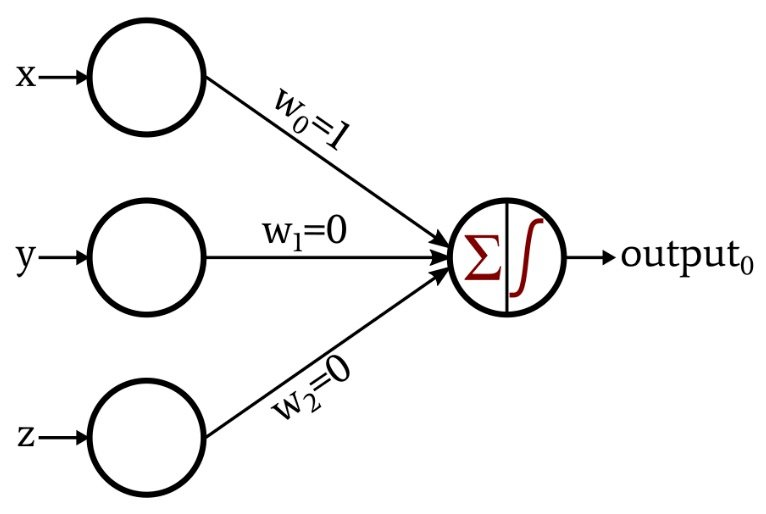
\includegraphics[width=0.4\textwidth,height=\textheight]{media/perceptron.jpeg}
\caption{\emph{Basic principle of Perceptron model.}}
\end{figure}

\begin{itemize}
\tightlist
\item
  1959: First application of neural networks from Stanford lab used to
  filter out noise in phone lines (still used to this day)
\item
  1969: Start of the AI ``dark ages'' where the Perceptron idea was
  killed by MIT (wrongly) followed by the cold war which made people
  overly-terrified of technology
\item
  1986: People got over this intellectual blockade and resumed research
  in AI and more specifically neural networks. This was catalyzed by the
  re-discovery of an older theory called \textbf{Backpropogation} which
  made neural networks much more applicable for larger, more diverse
  datasets.
\item
  2006: The development of the deep neural network (DNN), most common
  models created to date.
\end{itemize}

\hypertarget{what-led-to-the-development-and-use-of-them}{%
\subsubsection{What led to the development and use of
them?}\label{what-led-to-the-development-and-use-of-them}}

Originally, scientists were simply interested if they could recreate how
the human brain works; they really didn't have any desire to make this
concept much more than a concept. After WWII and Alan Turing's creation
of what would become the modern day computer, scientists that were able
to get their hands on this technology could turn it loose on whatever
they could imagine including early neural networks. For the next few
decades, the theory of artificial intelligence and neural networks
developed faster than technology could to support it until modern
computer processors and parallel computing caught up with the all of the
theory (Moore's law). Now the opposite seems to be true and computing
power is allowing for a lot more applications of neural networks and the
sky is the limit for real-world applications.

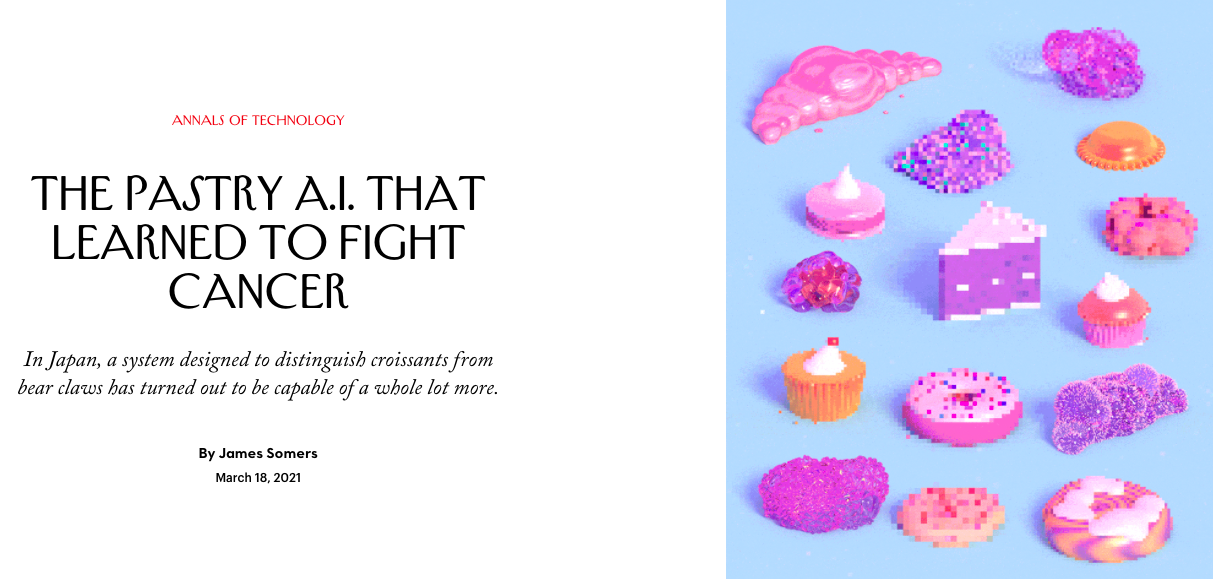
\includegraphics[width=0.6\textwidth,height=\textheight]{media/pastry.png}

\hypertarget{components-and-applications}{%
\section{Components and
applications}\label{components-and-applications}}

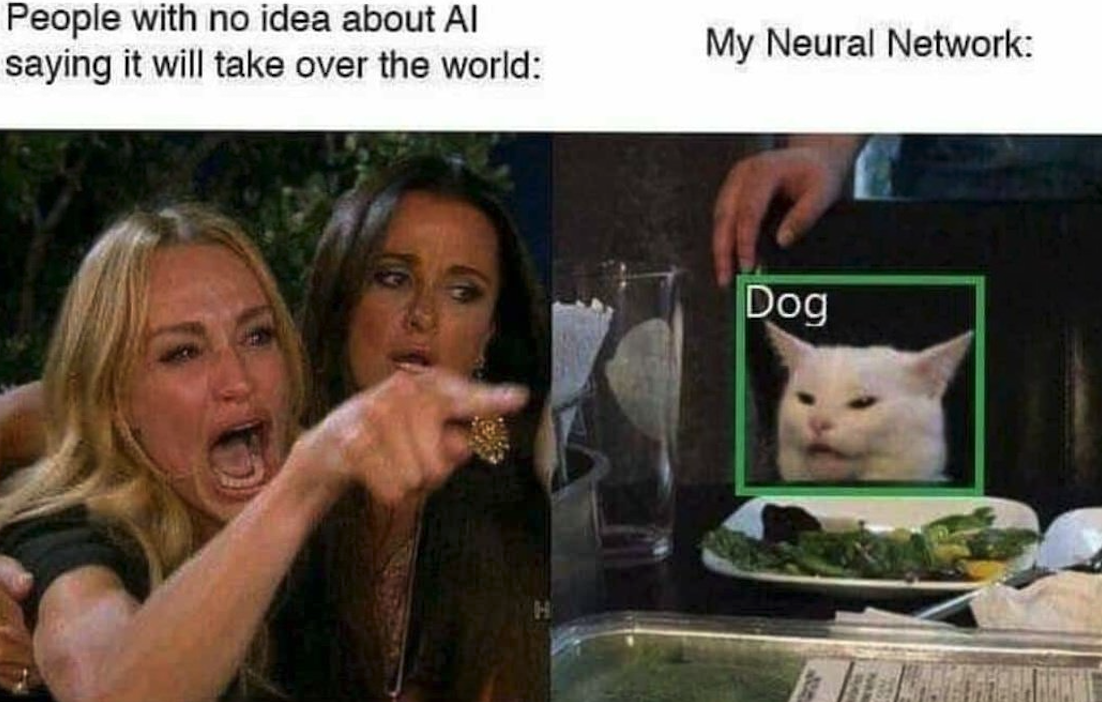
\includegraphics[width=0.6\textwidth,height=\textheight]{media/meme.png}

Neural networks are currently the fastest growing research topic (Google
scholar) as well as one of the most well-funded research areas. Most of
\emph{Nature's} most cited papers are based on neural network research.
They are capable of filling in analytical gaps where other statistical
methods simply fall short. While they process information the same way
our brains do, they are capable of finding patters that we simply are
not capable of.

\hypertarget{main-types-of-neural-networks}{%
\subsubsection{Main types of neural
networks}\label{main-types-of-neural-networks}}

\begin{enumerate}
\def\labelenumi{\arabic{enumi}.}
\tightlist
\item
  Artificial neural network (ANN)
\item
  Convolutional neural network (CNN)
\item
  Recurrent neural network (RNN)
\end{enumerate}

\hypertarget{components-and-function-of-neural-networks}{%
\subsubsection{Components and function of neural
networks}\label{components-and-function-of-neural-networks}}

Neural networks vary A LOT in structure, but most of them have
relatively similar components and building blocks.

\begin{figure}
\centering
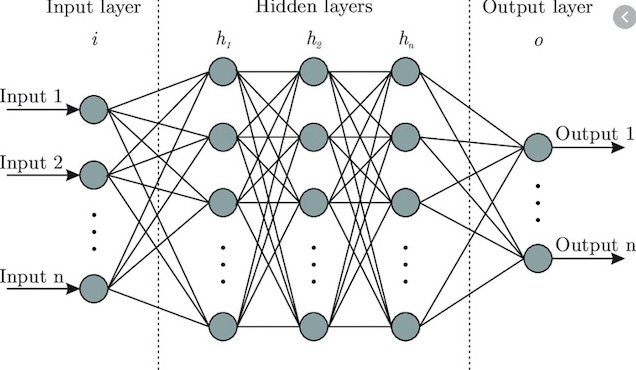
\includegraphics[width=0.7\textwidth,height=\textheight]{media/neuralNetDiagram.png}
\caption{\emph{Structure of a simple deep learning model}}
\end{figure}

\hypertarget{nodes}{%
\paragraph{Nodes}\label{nodes}}

A node is simply a container for a value with 1+ weighted input
connections, with the exception of the input layer which has yet to be
passed beyond the first input layer.

\hypertarget{input-layer}{%
\paragraph{Input layer}\label{input-layer}}

The input layer consist of whatever data you are choosing to help
predict your desired result. These come in many varieties and number of
input layers, but each input node always represents a single floating
point value. For the network we will be generating in R, it requires all
of our values be between 0 and 1 (requires scaling)

\hypertarget{hidden-layers}{%
\paragraph{Hidden layer(s)}\label{hidden-layers}}

Hidden layer(s) consist of a series of nodes that are used to take in a
weighted sum from a combination of nodes from the previous layer and
pass those values along to the following layer. This is the black box
area of neural networks; they can be very extensive and have many
different kinds of layers performing different computational tasks. This
is also where the term deep learning comes from, any ANN with multiple
hidden layers is considered a deep learning model.

\hypertarget{output-layer}{%
\paragraph{Output layer}\label{output-layer}}

This is our result. For classification-type models (i.e.~what do object
does the given input describe?), it will generate a value ranging from
0-1. In an ideal world, it would either be 0 or 1 each time, but it
usually varies and whichever value it is closest to is the generated
prediction. For numerical outputs, we have to rescale to get usable
output variables.

\hypertarget{weights}{%
\paragraph{Weights}\label{weights}}

A value that will change an input value to a node from the previous
layer depending upon its significance. Weights are multiplied by the
input value at your node.

\hypertarget{bias-value}{%
\paragraph{Bias value}\label{bias-value}}

Bias value is added to the above multiplication of the weight and input
at the node. You can think of this bias value as the equivalent of a
y-intercept in a linear model.

\hypertarget{assumptions-and-steps-for-building-one}{%
\section{Assumptions and steps for building
one}\label{assumptions-and-steps-for-building-one}}

\hypertarget{assumptions}{%
\subsubsection{Assumptions}\label{assumptions}}

\begin{itemize}
\tightlist
\item
  There really are none. You can pass any data into a neural network, it
  just needs to be structured first depending upon the model syntax; in
  our case all values need to be between 0-1.
\item
  They do tend to perform better when your output layer of your training
  dataset follows a uniform distribution.
\item
  Relationships are not always linear, the more input data you throw
  into a model the less often it is
\end{itemize}

\hypertarget{data-structure}{%
\subsubsection{Data structure}\label{data-structure}}

\begin{itemize}
\tightlist
\item
  Every model framework is slightly different
\item
  One consistent rule is that the data needs to be numeric

  \begin{itemize}
  \tightlist
  \item
    Easy to work around
  \end{itemize}
\item
  Understand your neural network application and create a training
  dataset with proper resolution
\item
  To properly train and test your model, it is recommended to take your
  data source and break it up 80/20 for training and testing data
\end{itemize}

\hypertarget{training-the-model}{%
\subsubsection{Training the model}\label{training-the-model}}

\begin{itemize}
\tightlist
\item
  Here we use a technique called \textbf{Backpropogation} (or something
  similar) to develop our model weights and bias values.
\item
  Backpropogation works with something commonly referred to as a cost or
  loss function in combination with another concept called
  \textbf{gradient descent}

  \begin{itemize}
  \tightlist
  \item
    Similar to how MCMC works to make these random guesses or jumps for
    posterior values
  \end{itemize}
\item
  Your model will start at your output layer with the ground-truthed
  training data you have provided and work backwards toward the input
  layer developing the weights and biases along the way
\item
  Each ``step'' in your backpropogation, the algorithm will alter the
  weights and biases to reflect an individual data point (i.e.~increase
  weights for a certain true value and decrease all others)
\item
  I could spend hours talking about this so I'll provide a couple links
  to YouTube videos on this process that are very helpful
\end{itemize}

\hypertarget{forward-pass-or-inference}{%
\subsubsection{Forward pass or
inference}\label{forward-pass-or-inference}}

Once we have successfully trained a properly fitted model, we then have
to implement it. In many data science cases this is relatively
straightforward, however if being implemented in real-time this can be a
very difficult and critical step to retrieve useful data. This process
is usually referred to as your forward pass or \textbf{inference} step.
You may see models referred to as ``forward feeding'' and this simply
means that data is moving from your input to your output layer.

\hypertarget{issues-with-neural-networks}{%
\section{Issues with neural
networks}\label{issues-with-neural-networks}}

While neural networks are incredibly powerful and useful tools, they
come with their caveats. \#\#\# Overfitting This is one area of
similarity that neural networks share with other models. Overfitting is
a very common issue encountered while training a neural network, however
it is rather easily avoidable if properly monitored and input parameters
are adjusted accordingly. - Don't train model for excessive amount of
steps/epochs - Play around with your learning rate: simply models don't
require a slow learning rate - If all else fails, try different
backpropogation methods

\begin{figure}
\centering
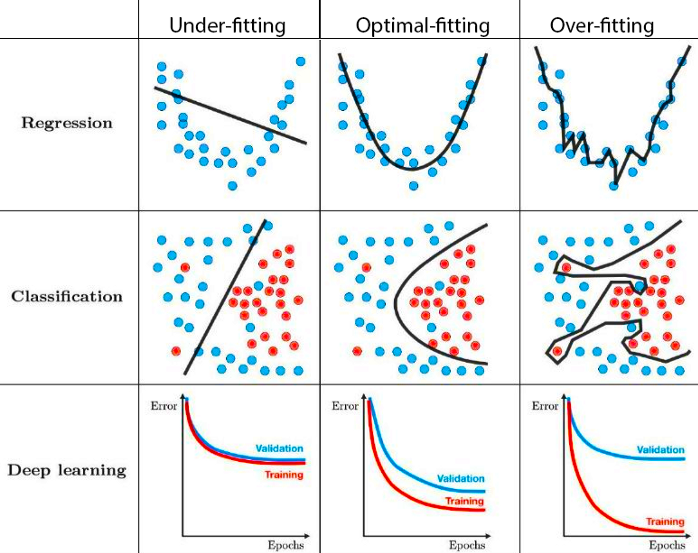
\includegraphics{media/overfittingDiagram.png}
\caption{\emph{Useful diagram depicting overfitting of various models}}
\end{figure}

\hypertarget{a-lot-of-unknowns}{%
\subsubsection{A lot of unknowns}\label{a-lot-of-unknowns}}

\begin{itemize}
\tightlist
\item
  With very simply models, it can be relatively easy to decipher what
  the model is thinking.
\item
  Once you work up to larger models all hope is lost of trying to figure
  out what the computer is learning.
\item
  Currently not a very accepted method of analysis in a lot of fields
\end{itemize}

\hypertarget{collecting-sufficient-training-data-can-be-arduous}{%
\subsubsection{Collecting sufficient training data can be
arduous}\label{collecting-sufficient-training-data-can-be-arduous}}

\begin{itemize}
\tightlist
\item
  Depending upon what datasets you work with, collecting and formatting
  training data can be very tedious (i.e.~image annotation for CNNs)
\item
  Sometimes you are simply given bad data and this is very problematic
\end{itemize}

\hypertarget{lets-do-some-coding}{%
\section{Let's do some coding}\label{lets-do-some-coding}}

Let's start with a simple example from the iris dataset (sorry)

\hypertarget{load-packages}{%
\subsubsection{Load packages}\label{load-packages}}

\begin{Shaded}
\begin{Highlighting}[]
\FunctionTok{library}\NormalTok{(dplyr)}
\FunctionTok{library}\NormalTok{(neuralnet)}
\FunctionTok{library}\NormalTok{(stringr)}
\FunctionTok{library}\NormalTok{(LaplacesDemon)}
\end{Highlighting}
\end{Shaded}

\hypertarget{load-and-visualize-data}{%
\subsubsection{Load and visualize data}\label{load-and-visualize-data}}

\begin{Shaded}
\begin{Highlighting}[]
\FunctionTok{head}\NormalTok{(iris)}
\end{Highlighting}
\end{Shaded}

\begin{verbatim}
##   Sepal.Length Sepal.Width Petal.Length Petal.Width Species
## 1          5.1         3.5          1.4         0.2  setosa
## 2          4.9         3.0          1.4         0.2  setosa
## 3          4.7         3.2          1.3         0.2  setosa
## 4          4.6         3.1          1.5         0.2  setosa
## 5          5.0         3.6          1.4         0.2  setosa
## 6          5.4         3.9          1.7         0.4  setosa
\end{verbatim}

\begin{Shaded}
\begin{Highlighting}[]
\FunctionTok{summary}\NormalTok{(iris}\SpecialCharTok{$}\NormalTok{Species) }\CommentTok{\#this is our output layer, or what we are predicting}
\end{Highlighting}
\end{Shaded}

\begin{verbatim}
##     setosa versicolor  virginica 
##         50         50         50
\end{verbatim}

\hypertarget{format-the-data}{%
\subsubsection{Format the data}\label{format-the-data}}

\begin{Shaded}
\begin{Highlighting}[]
\NormalTok{cleanedIris }\OtherTok{\textless{}{-}} \FunctionTok{model.matrix}\NormalTok{(}\SpecialCharTok{\textasciitilde{}}\NormalTok{ Sepal.Length }\SpecialCharTok{+}\NormalTok{ Sepal.Width }\SpecialCharTok{+}\NormalTok{ Petal.Length }\SpecialCharTok{+}\NormalTok{ Petal.Width }\SpecialCharTok{+}\NormalTok{ Species,}\AttributeTok{data=}\NormalTok{iris)}
\NormalTok{cleanedIris }\OtherTok{\textless{}{-}}\NormalTok{ cleanedIris}\SpecialCharTok{/}\FunctionTok{max}\NormalTok{(cleanedIris)}
\FunctionTok{head}\NormalTok{(cleanedIris)}
\end{Highlighting}
\end{Shaded}

\begin{verbatim}
##   (Intercept) Sepal.Length Sepal.Width Petal.Length Petal.Width
## 1   0.1265823    0.6455696   0.4430380    0.1772152  0.02531646
## 2   0.1265823    0.6202532   0.3797468    0.1772152  0.02531646
## 3   0.1265823    0.5949367   0.4050633    0.1645570  0.02531646
## 4   0.1265823    0.5822785   0.3924051    0.1898734  0.02531646
## 5   0.1265823    0.6329114   0.4556962    0.1772152  0.02531646
## 6   0.1265823    0.6835443   0.4936709    0.2151899  0.05063291
##   Speciesversicolor Speciesvirginica
## 1                 0                0
## 2                 0                0
## 3                 0                0
## 4                 0                0
## 5                 0                0
## 6                 0                0
\end{verbatim}

This dataframe snippet shows the format necessary for the neuralnet()
function in R. To properly process the data, all of the values need to
be between 0 and 1.

\hypertarget{visualize-the-neuralnet}{%
\subsubsection{Visualize the neuralnet}\label{visualize-the-neuralnet}}

\begin{Shaded}
\begin{Highlighting}[]
\NormalTok{irisNN }\OtherTok{\textless{}{-}} \FunctionTok{neuralnet}\NormalTok{(Speciesversicolor}\SpecialCharTok{+}\NormalTok{Speciesvirginica}\SpecialCharTok{\textasciitilde{}}\NormalTok{Sepal.Length}\SpecialCharTok{+}\NormalTok{Sepal.Width}\SpecialCharTok{+}\NormalTok{Petal.Length}\SpecialCharTok{+}\NormalTok{Petal.Width,}
\NormalTok{                    cleanedIris, }\AttributeTok{hidden=}\DecValTok{1}\NormalTok{,}\AttributeTok{algorithm=}\StringTok{"rprop+"}\NormalTok{,}
                    \AttributeTok{learningrate=}\FloatTok{0.01}\NormalTok{, }\AttributeTok{linear.output=}\NormalTok{F)}
\FunctionTok{plot}\NormalTok{(irisNN)}
\end{Highlighting}
\end{Shaded}

While the iris dataset is painful to look at, it is very useful for
generating a strong correlation and creating a simple, interpretable
model. For now, lets not worry about the forward pass portion. So let's
walk through this a bit.

\begin{figure}
\centering
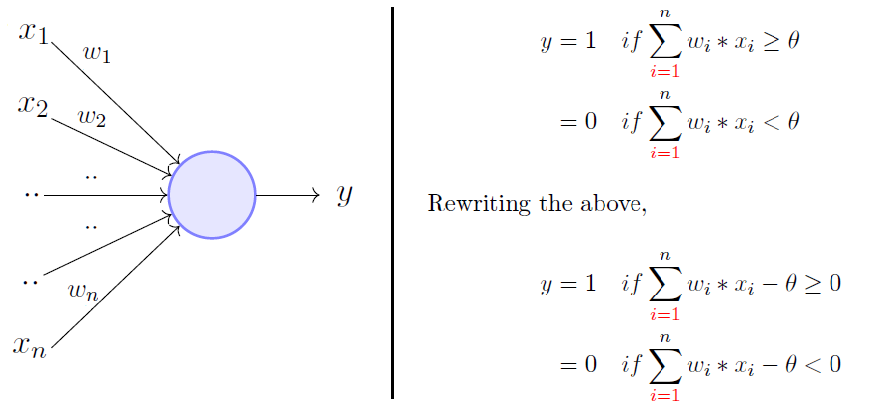
\includegraphics[width=0.6\textwidth,height=\textheight]{media/perceptronModel.png}
\caption{\emph{Formula}}
\end{figure}

\hypertarget{lets-play-around-with-some-different-data}{%
\subsection{Let's play around with some different
data}\label{lets-play-around-with-some-different-data}}

Thanks to some friends that work over at the Nevada Humane Society, I
was able to get my hands on their largescale dataset
(n\textgreater10000) for animal adoptions. This provided a good
opportunity to create a neural network to predict residency times for
incoming animals to the shelter, useful for understanding resource
allocation for shelter pets. So lets look at some data.

\hypertarget{importing-data}{%
\subsubsection{Importing data}\label{importing-data}}

\begin{Shaded}
\begin{Highlighting}[]
\NormalTok{df }\OtherTok{\textless{}{-}} \FunctionTok{read.csv}\NormalTok{(}\StringTok{\textquotesingle{}/Users/keaneflynn/Downloads/R{-}Program/NRES\_746/NeuralNetworks/nhseData.csv\textquotesingle{}}\NormalTok{)}
\NormalTok{df }\OtherTok{\textless{}{-}}\NormalTok{ df[}\SpecialCharTok{!}\FunctionTok{duplicated}\NormalTok{(df[,}\FunctionTok{c}\NormalTok{(}\StringTok{"Name"}\NormalTok{, }\StringTok{"Species"}\NormalTok{)]),] }
\FunctionTok{head}\NormalTok{(df)}
\end{Highlighting}
\end{Shaded}

\begin{verbatim}
##    Created.Date    Name Species              Primary.Breed    Sex Age..Months.
## 1    03/13/2020    Luna     Dog        Pinscher, Miniature Female          146
## 4    01/30/2020   BUDDY     Dog Terrier, Yorkshire, Yorkie   Male          122
## 5    03/05/2020  BUDDAH     Cat          Domestic Longhair Female           74
## 7    02/05/2020   SASSY     Dog                 Rottweiler Female          106
## 8    01/27/2020 Biscuit     Dog      Terrier, Jack Russell Female          188
## 10   02/07/2020 Frankie     Dog                     Beagle   Male          183
##                 Age.Group Primary.Color Days.in.Custody Days.on.Site
## 1        Senior (8+years)         Black               1            1
## 4        Senior (8+years)         Brown               1            1
## 5  Adult Cat (5-10 years)         White               3            3
## 7        Senior (8+years)         Black               1            1
## 8        Senior (8+years)         White               1            1
## 10       Senior (8+years)         Brown               1            1
##    Current.Weight Attributes
## 1         9.4 lbs  Angel Pet
## 4                           
## 5       11.38 lbs           
## 7                           
## 8        25.4 lbs           
## 10         31 lbs
\end{verbatim}

\hypertarget{specific-data-point}{%
\subsubsection{Specific data point}\label{specific-data-point}}

\begin{Shaded}
\begin{Highlighting}[]
\NormalTok{df }\SpecialCharTok{\%\textgreater{}\%} \FunctionTok{filter}\NormalTok{(Name}\SpecialCharTok{==}\StringTok{"Donut"}\NormalTok{) }\CommentTok{\#This is my pup}
\end{Highlighting}
\end{Shaded}

\begin{verbatim}
##   Created.Date  Name Species              Primary.Breed  Sex Age..Months.
## 1   07/15/2021 Donut     Dog Terrier, American Pit Bull Male            7
##                      Age.Group Primary.Color Days.in.Custody Days.on.Site
## 1 Adult Dog (5 months-8 years)         Black             108            8
##   Current.Weight
## 1       56.5 lbs
##                                                                                      Attributes
## 1 D2D Required,Heart Murmur,Kids under 6 meet first,Unavailable - waiting for medical procedure
\end{verbatim}

\hypertarget{regrouping-data}{%
\subsubsection{Regrouping data}\label{regrouping-data}}

\begin{Shaded}
\begin{Highlighting}[]
\NormalTok{df}\SpecialCharTok{$}\NormalTok{Age.Group }\OtherTok{\textless{}{-}} \FunctionTok{str\_remove\_all}\NormalTok{(df}\SpecialCharTok{$}\NormalTok{Age.Group,}\StringTok{" }\SpecialCharTok{\textbackslash{}\textbackslash{}}\StringTok{(.*?}\SpecialCharTok{\textbackslash{}\textbackslash{}}\StringTok{)"}\NormalTok{)}
\NormalTok{df}\SpecialCharTok{$}\NormalTok{Age.Group }\OtherTok{\textless{}{-}} \FunctionTok{str\_replace\_all}\NormalTok{(df}\SpecialCharTok{$}\NormalTok{Age.Group,}\StringTok{"Juvenile|Kitten|Puppy|Unweaned"}\NormalTok{,}\StringTok{"juvenile"}\NormalTok{)}
\NormalTok{df}\SpecialCharTok{$}\NormalTok{Age.Group }\OtherTok{\textless{}{-}} \FunctionTok{str\_replace\_all}\NormalTok{(df}\SpecialCharTok{$}\NormalTok{Age.Group,}\StringTok{"Adult Cat|Adult Dog|Adult|Young adult"}\NormalTok{,}\StringTok{"adult"}\NormalTok{)}
\NormalTok{df}\SpecialCharTok{$}\NormalTok{Age.Group }\OtherTok{\textless{}{-}} \FunctionTok{str\_replace\_all}\NormalTok{(df}\SpecialCharTok{$}\NormalTok{Age.Group,}\StringTok{"Senior"}\NormalTok{,}\StringTok{"senior"}\NormalTok{)}

\NormalTok{df}\SpecialCharTok{$}\NormalTok{Current.Weight }\OtherTok{\textless{}{-}} \FunctionTok{as.numeric}\NormalTok{(}\FunctionTok{str\_extract\_all}\NormalTok{(df}\SpecialCharTok{$}\NormalTok{Current.Weight,}\StringTok{"}\SpecialCharTok{\textbackslash{}\textbackslash{}}\StringTok{d\{0,3\}.}\SpecialCharTok{\textbackslash{}\textbackslash{}}\StringTok{d\{1,2\}"}\NormalTok{))}

\NormalTok{df}\SpecialCharTok{$}\NormalTok{Sex }\OtherTok{\textless{}{-}} \FunctionTok{str\_replace\_all}\NormalTok{(df}\SpecialCharTok{$}\NormalTok{Sex,}\StringTok{"Male"}\NormalTok{,}\StringTok{"male"}\NormalTok{)}
\NormalTok{df}\SpecialCharTok{$}\NormalTok{Sex }\OtherTok{\textless{}{-}} \FunctionTok{str\_replace\_all}\NormalTok{(df}\SpecialCharTok{$}\NormalTok{Sex,}\StringTok{"Female"}\NormalTok{,}\StringTok{"female"}\NormalTok{)}
\NormalTok{df}\SpecialCharTok{$}\NormalTok{Sex }\OtherTok{\textless{}{-}} \FunctionTok{str\_replace\_all}\NormalTok{(df}\SpecialCharTok{$}\NormalTok{Sex,}\StringTok{"Unknown"}\NormalTok{,}\StringTok{"unknown"}\NormalTok{)}

\NormalTok{df}\SpecialCharTok{$}\NormalTok{Species }\OtherTok{\textless{}{-}} \FunctionTok{str\_replace\_all}\NormalTok{(df}\SpecialCharTok{$}\NormalTok{Species,}\StringTok{"Bird, Unspecified|Chicken, Domestic|Conure, Unspecified|Parakeet, Common|Parakeet, Unspecified"}\NormalTok{,}\StringTok{"bird"}\NormalTok{)}
\NormalTok{df}\SpecialCharTok{$}\NormalTok{Species }\OtherTok{\textless{}{-}} \FunctionTok{str\_replace\_all}\NormalTok{(df}\SpecialCharTok{$}\NormalTok{Species,}\StringTok{"Lizard, Unspecified|Snake, Python Unspecified|Tortoise, Unspecified|Turtle, Red{-}Eared Slider|Turtle, Unspecified"}\NormalTok{,}\StringTok{"reptile"}\NormalTok{)}
\NormalTok{df}\SpecialCharTok{$}\NormalTok{Species }\OtherTok{\textless{}{-}} \FunctionTok{str\_replace\_all}\NormalTok{(df}\SpecialCharTok{$}\NormalTok{Species,}\StringTok{"Chinchilla|Ferret|Guinea Pig|Hamster, Dwarf|Hamster, Unspecified|Hedgehog|Mouse, Little Pocket|Mouse, Unspecified|Rabbit, Domestic|Rat, Unspecified|Sugar Glider"}\NormalTok{,}\StringTok{"small\_mammal"}\NormalTok{)}
\NormalTok{df}\SpecialCharTok{$}\NormalTok{Species }\OtherTok{\textless{}{-}} \FunctionTok{str\_replace\_all}\NormalTok{(df}\SpecialCharTok{$}\NormalTok{Species,}\StringTok{"Dog"}\NormalTok{,}\StringTok{"dog"}\NormalTok{)}
\NormalTok{df}\SpecialCharTok{$}\NormalTok{Species }\OtherTok{\textless{}{-}} \FunctionTok{str\_replace\_all}\NormalTok{(df}\SpecialCharTok{$}\NormalTok{Species,}\StringTok{"Cat"}\NormalTok{,}\StringTok{"cat"}\NormalTok{)}
\end{Highlighting}
\end{Shaded}

\hypertarget{final-dataframe-cleansing}{%
\subsubsection{Final dataframe
cleansing}\label{final-dataframe-cleansing}}

\begin{Shaded}
\begin{Highlighting}[]
\NormalTok{df }\OtherTok{\textless{}{-}}\NormalTok{ dplyr}\SpecialCharTok{::}\FunctionTok{rename}\NormalTok{(df, }\FunctionTok{c}\NormalTok{(}\AttributeTok{species =}\NormalTok{ Species,}
                          \AttributeTok{breed =}\NormalTok{ Primary.Breed,}
                          \AttributeTok{sex =}\NormalTok{ Sex,}
                          \AttributeTok{age =}\NormalTok{ Age..Months.,}
                          \AttributeTok{age\_group =}\NormalTok{ Age.Group,}
                          \AttributeTok{weight\_lbs =}\NormalTok{ Current.Weight,}
                          \AttributeTok{custody\_period =}\NormalTok{ Days.in.Custody)) }\SpecialCharTok{\%\textgreater{}\%}
  \FunctionTok{select}\NormalTok{(species,sex,age\_group,age,weight\_lbs,custody\_period) }\SpecialCharTok{\%\textgreater{}\%} 
  \FunctionTok{na.omit}\NormalTok{()}
\FunctionTok{rownames}\NormalTok{(df) }\OtherTok{\textless{}{-}} \DecValTok{1}\SpecialCharTok{:}\FunctionTok{nrow}\NormalTok{(df)}
\NormalTok{df\_check }\OtherTok{\textless{}{-}}\NormalTok{ df[}\SpecialCharTok{{-}}\FunctionTok{c}\NormalTok{(}\DecValTok{2860}\NormalTok{,}\DecValTok{755}\NormalTok{,}\DecValTok{5856}\NormalTok{,}\DecValTok{4709}\NormalTok{,}\DecValTok{5189}\NormalTok{),] }\CommentTok{\#removing some outliers that are annoying me}
\FunctionTok{head}\NormalTok{(df\_check)}
\end{Highlighting}
\end{Shaded}

\begin{verbatim}
##   species    sex age_group age weight_lbs custody_period
## 1     dog female    senior 146       9.40              1
## 2     cat female     adult  74      11.38              3
## 3     dog female    senior 188      25.40              1
## 4     dog   male    senior 183      31.00              1
## 5     cat female     adult  99       8.40              1
## 6     dog female     adult  75      70.80             28
\end{verbatim}

Here we have a cleaner, more interpretable dataframe, where we can see
the basis of our input layer and our output layer. Depending upon the
dataset, adding more input layers can improve model accuracy but the
hidden layers tend to have more relevance in model performance.

\hypertarget{formatting-the-dataframe-for-the-neuralnet-package}{%
\subsubsection{Formatting the dataframe for the neuralnet()
package}\label{formatting-the-dataframe-for-the-neuralnet-package}}

\begin{Shaded}
\begin{Highlighting}[]
\NormalTok{formatted\_df }\OtherTok{\textless{}{-}} \FunctionTok{model.matrix}\NormalTok{(}\SpecialCharTok{\textasciitilde{}}\NormalTok{ species }\SpecialCharTok{+}\NormalTok{ sex }\SpecialCharTok{+}\NormalTok{ age\_group }\SpecialCharTok{+}\NormalTok{ age }\SpecialCharTok{+}\NormalTok{ weight\_lbs }\SpecialCharTok{+}\NormalTok{ custody\_period,}\AttributeTok{data=}\NormalTok{df\_check)}
\NormalTok{maxVal }\OtherTok{\textless{}{-}} \FunctionTok{max}\NormalTok{(formatted\_df) }\CommentTok{\#variable stored to unscale our dataframe, important for later}
\NormalTok{formatted\_df }\OtherTok{\textless{}{-}}\NormalTok{ formatted\_df}\SpecialCharTok{/}\NormalTok{maxVal}
\FunctionTok{head}\NormalTok{(formatted\_df)}
\end{Highlighting}
\end{Shaded}

\begin{verbatim}
##   (Intercept)  speciesdog speciesreptile speciessmall_mammal     sexmale
## 1 0.001636661 0.001636661              0                   0 0.000000000
## 2 0.001636661 0.000000000              0                   0 0.000000000
## 3 0.001636661 0.001636661              0                   0 0.000000000
## 4 0.001636661 0.001636661              0                   0 0.001636661
## 5 0.001636661 0.000000000              0                   0 0.000000000
## 6 0.001636661 0.001636661              0                   0 0.000000000
##   sexunknown age_groupjuvenile age_groupsenior       age weight_lbs
## 1          0                 0     0.001636661 0.2389525 0.01538462
## 2          0                 0     0.000000000 0.1211129 0.01862520
## 3          0                 0     0.001636661 0.3076923 0.04157119
## 4          0                 0     0.001636661 0.2995090 0.05073650
## 5          0                 0     0.000000000 0.1620295 0.01374795
## 6          0                 0     0.000000000 0.1227496 0.11587561
##   custody_period
## 1    0.001636661
## 2    0.004909984
## 3    0.001636661
## 4    0.001636661
## 5    0.001636661
## 6    0.045826514
\end{verbatim}

\hypertarget{breaking-up-into-training-and-testing-data}{%
\subsubsection{Breaking up into training and testing
data}\label{breaking-up-into-training-and-testing-data}}

Recall that we need 80\% of our data for training our model and 20\% for
testing, so lets go ahead and break it up accordingly and randomly to
avoid accidentally fitting our model to specific attributes.

\begin{Shaded}
\begin{Highlighting}[]
\FunctionTok{set.seed}\NormalTok{(}\DecValTok{70}\NormalTok{) }\CommentTok{\#sample pseudo{-}randomly for replication sake}
\NormalTok{sampleSize }\OtherTok{\textless{}{-}} \FunctionTok{round}\NormalTok{(}\FunctionTok{nrow}\NormalTok{(formatted\_df)}\SpecialCharTok{*}\FloatTok{0.8}\NormalTok{) }\CommentTok{\#split up dataset 80/20}
\NormalTok{rowIndex }\OtherTok{\textless{}{-}} \FunctionTok{sample}\NormalTok{(}\FunctionTok{seq}\NormalTok{(}\FunctionTok{nrow}\NormalTok{(formatted\_df)),}\AttributeTok{size=}\NormalTok{sampleSize)}

\NormalTok{training\_data }\OtherTok{\textless{}{-}}\NormalTok{ formatted\_df[rowIndex,] }\CommentTok{\#what will be passed into the model training function}
\NormalTok{testing\_data }\OtherTok{\textless{}{-}}\NormalTok{  formatted\_df[}\SpecialCharTok{{-}}\NormalTok{rowIndex,]}
\NormalTok{groundtruth\_data }\OtherTok{\textless{}{-}}\NormalTok{ testing\_data[,}\DecValTok{11}\NormalTok{]}\SpecialCharTok{*}\NormalTok{maxVal}
\end{Highlighting}
\end{Shaded}

\hypertarget{train-and-visualize-our-new-network-for-pet-adoptions}{%
\subsubsection{Train and visualize our new network for pet
adoptions}\label{train-and-visualize-our-new-network-for-pet-adoptions}}

\begin{Shaded}
\begin{Highlighting}[]
\NormalTok{nn }\OtherTok{\textless{}{-}} \FunctionTok{neuralnet}\NormalTok{(custody\_period}\SpecialCharTok{\textasciitilde{}}\NormalTok{speciesdog}\SpecialCharTok{+}\NormalTok{speciesreptile}\SpecialCharTok{+}\NormalTok{speciessmall\_mammal}\SpecialCharTok{+}\NormalTok{sexmale}\SpecialCharTok{+}\NormalTok{sexunknown}\SpecialCharTok{+}\NormalTok{age\_groupjuvenile}\SpecialCharTok{+}\NormalTok{age\_groupsenior}\SpecialCharTok{+}\NormalTok{age}\SpecialCharTok{+}\NormalTok{weight\_lbs,}
\NormalTok{                training\_data,}
                \AttributeTok{hidden=}\FunctionTok{c}\NormalTok{(}\DecValTok{5}\NormalTok{,}\DecValTok{2}\NormalTok{), }\AttributeTok{learningrate=}\FloatTok{0.01}\NormalTok{,  }
                \AttributeTok{linear.output=}\NormalTok{T)}
\FunctionTok{plot}\NormalTok{(nn)}
\end{Highlighting}
\end{Shaded}

\hypertarget{cool-applications-in-ecology}{%
\section{Cool applications in
ecology}\label{cool-applications-in-ecology}}

\hypertarget{additional-sources-of-information}{%
\subsubsection{Additional sources of
information}\label{additional-sources-of-information}}

\hypertarget{backpropogation}{%
\paragraph{Backpropogation}\label{backpropogation}}

\href{https://www.youtube.com/watch?v=Ilg3gGewQ5U}{Backpropogation
Overview}
\href{https://www.youtube.com/watch?v=tIeHLnjs5U8}{Backpropogation
Calculus}

\hypertarget{citations}{%
\subsubsection{Citations}\label{citations}}

\begin{enumerate}
\def\labelenumi{\arabic{enumi}.}
\tightlist
\item
  Hecht-Nielsen, R. (1992). Theory of the backpropagation neural
  network. In Neural networks for perception (pp.~65-93). Academic
  Press.
\item
\end{enumerate}

\end{document}
